% Template for Cogsci submission with R Markdown

% Stuff changed from original Markdown PLOS Template
\documentclass[10pt, letterpaper]{article}

\usepackage{cogsci}
\usepackage{pslatex}
\usepackage{float}
\usepackage{caption}

% amsmath package, useful for mathematical formulas
\usepackage{amsmath}

% amssymb package, useful for mathematical symbols
\usepackage{amssymb}

% hyperref package, useful for hyperlinks
\usepackage{hyperref}

% graphicx package, useful for including eps and pdf graphics
% include graphics with the command \includegraphics
\usepackage{graphicx}

% Sweave(-like)
\usepackage{fancyvrb}
\DefineVerbatimEnvironment{Sinput}{Verbatim}{fontshape=sl}
\DefineVerbatimEnvironment{Soutput}{Verbatim}{}
\DefineVerbatimEnvironment{Scode}{Verbatim}{fontshape=sl}
\newenvironment{Schunk}{}{}
\DefineVerbatimEnvironment{Code}{Verbatim}{}
\DefineVerbatimEnvironment{CodeInput}{Verbatim}{fontshape=sl}
\DefineVerbatimEnvironment{CodeOutput}{Verbatim}{}
\newenvironment{CodeChunk}{}{}

% cite package, to clean up citations in the main text. Do not remove.
\usepackage{apacite}

% KM added 1/4/18 to allow control of blind submission


\usepackage{color}

% Use doublespacing - comment out for single spacing
%\usepackage{setspace}
%\doublespacing


% % Text layout
% \topmargin 0.0cm
% \oddsidemargin 0.5cm
% \evensidemargin 0.5cm
% \textwidth 16cm
% \textheight 21cm

\title{Frequency-dependent regularization arises from a noisy-channel
processing model}


\author{{\large \bf Zachary Houghton (znhoughton@ucdavis.edu)} \\ Department of Linguistics, 1 Shields Avenue \\ Davis, CA 95616 USA \AND {\large \bf Emily Morgan (eimorgan@ucdavis.edu)} \\ Department of Linguistics, 1 Shields Avenue \\ Davis, CA 95616 USA}

\newlength{\cslhangindent}
\setlength{\cslhangindent}{1.5em}
\newenvironment{CSLReferences}%
  {}%
  {\par}

\begin{document}

\maketitle

\begin{abstract}
Language often has different ways to express the same or similar
meanings. Despite this, however, people seem to have preferences for
some ways over others. For example, people overwhelmingly prefer
\emph{bread and butter} to \emph{butter and bread}. Previous research
has demonstrated that these ordering preferences grow stronger with
frequency (i.e., frequency-dependent regularization). In this paper we
demonstrate that this frequency-dependent regularization can be
accounted for by noisy-channel processing models (e.g., Gibson, Bergen,
\& Piantadosi, 2013; Levy, 2008). We also show that this regularization
can only be accounted for if the listener infers more noise than the
speaker produces. Finally, we show that the model can account for the
language-wide distribution of binomial ordering preferences.

\textbf{Keywords:}
Frequency-dependent regularization; Noisy-channel processing;
Psycholinguistics.
\end{abstract}

\hypertarget{introduction}{%
\section{Introduction}\label{introduction}}

Speakers are often confronted with many different ways to express the
same meaning. A customer might ask whether a store sells ``radios and
televisions'', but they could have just as naturally asked whether the
store sells ``televisions and radios.'' However, despite conveying the
same meaning, speakers sometimes have strong preferences for one choice
over competing choices (e.g., preference for \emph{men and women} over
\emph{women and men}, Benor \& Levy, 2006; Morgan \& Levy, 2016a). These
preferences are driven to some extent by generative preferences (e.g.,
preference for short words before long words), however they are
sometimes violated by idiosyncratic preferences (e.g., \emph{ladies and
gentlemen} preferred despite a general men-before-women generative
preference, Morgan \& Levy, 2016b).

Interestingly, ordering preferences for certain constructions, such as
binomial expressions, are often more extreme for higher frequency items
(e.g., \emph{bread and butter}). That is, higher-frequency items
typically have more polarized preferences (Liu \& Morgan, 2020, 2021;
Morgan \& Levy, 2015, 2016b, 2016a). This phenomenon is called
\emph{Frequency-dependent regularization}, and while there is evidence
of it in several different constructions, it is still unclear what
processeses this phenomenon is driven by. For example, it could be a
consequence of learning processes or a consequence of sentence
processing more broadly. In the present paper we examine whether a
noisy-channel processing model (Gibson et al., 2013) combined with
transmission across generations (Reali \& Griffiths, 2009) can account
for frequency-dependent regularization.

\hypertarget{frequency-dependent-regularization}{%
\subsection{Frequency-dependent
regularization}\label{frequency-dependent-regularization}}

Frequency-dependent regularization has been documented for a variety of
different constructions in English (Liu \& Morgan, 2020, 2021; Morgan \&
Levy, 2015, 2016b). For example, Morgan \& Levy (2015) demonstrated that
more frequent binomial expressions (e.g., \emph{bread and butter}) are
more strongly regularized (i.e., are preferred in one order
overwhelmingly more than the alternative). These ordering preferences
are also not simply a result of abstract ordering preferences (e.g.,
short words before long words, Morgan \& Levy, 2016a).

Additionally, Liu \& Morgan (2020) demonstrated this effect holds true
for the dative alternation in English (e.g., \emph{give} \emph{the ball
to him}~vs \emph{give him the ball}). Specifically, they demonstrated
higher frequency verbs have more polarized preferences with respect to
the dative alternation. Similarly, Liu \& Morgan (2021) showed that
Adjective-Adjective-Noun orderings also show frequency-dependent
regularization. That is, adjective-adjective-Nouns with higher overall
frequencies show stronger ordering preferences, even after taking into
account generative preferences of adjective orderings.

How does this polarization for high-frequency items arise? One
possibility is that it occurs as a consequence of imperfect transmission
between generations. For example, as speakers transmit the language from
one generation to the next, it is possible that the next generation may
infer the probability of each ordering imperfectly. Indeed, Morgan \&
Levy (2016b) demonstrated this possibility in an iterated-learning
paradigm. They showed that frequency-dependent regularization can arise
from an interaction between a frequency-independent bias and
transmission across generations. Specifically, they used an iterated
learning paradigm (following Reali \& Griffiths, 2009) and demonstrated
that by introducing a frequency-independent regularization bias, after
several generations the model predicted frequency-\emph{dependent}
regularization. However, it is unclear what process in language is
analogous to the frequency-independent bias.

\hypertarget{noisy-channel-processing}{%
\subsection{Noisy-channel Processing}\label{noisy-channel-processing}}

One possibility is that frequency-dependent regularization arises as a
product of noisy-channel processing (Gibson et al., 2013). Listeners are
confronted with a great deal of noise in the form of perception errors
(e.g., a noisy environment) and even production errors (speakers don't
always say what they intended to, Gibson et al., 2013). In order to
overcome these errors, a processing system must take into account the
noise of the system.

Indeed, there is evidence that our processing system does take noise
into account. For example, Ganong (1980) found that people will process
a non-word as being a word under noisy conditions. Additionally, Albert
Felty, Buchwald, Gruenenfelder, \& Pisoni (2013) demonstrated that when
listeners do misperceive a word, the word that they believe to have
heard tends to be higher frequency than the target word. Further, Keshev
\& Meltzer-Asscher (2021) found that in Arabic, readers will even
process ambiguous subject/object relative clauses as the more frequent
interpretation, even if this interpretation compromises subject-verb
agreement. These results taken together suggests that misperceptions may
sometimes actually be a consequence of noisy-channel processing (rather
than a failure of our perceptual system).\footnote{Changing \(\nu\) does
  not qualitatively change the pattern of the results for any
  simulations in the paper, as long as it's greater than 2.}

In order to account for findings like these, Gibson et al. (2013)
developed a computational model that demonstrated how a system might
take into account noise (see Levy, 2008 for a similar approach).
Specifically, their model operationalizes noisy-channel processing as a
Bayesian process where a listener estimates the probability that their
perception matches the speaker's intended utterance. Specifically, this
is operationlized as being proportional to the prior probability of the
intended utterance multiplied by the probability of the intended
utterance being corrupted to the perceived utterance (See Equation
\ref{eq:gibsonnoisy}):

\begin{equation}
\label{eq:gibsonnoisy}
P(S_i|S_p) \propto P(S_i) P(S_i \to S_p)
\end{equation}

where \(P(S_i|S_p)\) is the probability that the intended utterance was
actually the utterance that was perceived, \(P(S_i)\) is the prior
probability of the intended utterance, and \(P(S_i \to S_p)\) is the
probability that the intended utterance was corrupted by noise.

Gibson et al. (2013)'s model made a variety of interesting predictions.
For example, the model predicted that when people are presented with an
implausible sentence (e.g., \emph{the mother gave the candle the
daughter}), they should be more likely to interpret the plausible
version of the sentence (e.g., \emph{the mother gave the candle to the
daughter}) if there is increased noise (e.g., by adding syntactic errors
to the filler items, such as a deleted function word). Their model also
predicted that increasing the likelihood of implausible events (e.g., by
adding more filler items that were implausible, such as \emph{the girl
was kicked by the ball}) should increase the rate of implausible
interpretations of the sentence. Interestingly both of these results
were born out in their experimental data, suggesting that humans do
utilize a noisy-channel system in processing.

\hypertarget{present-study}{%
\subsection{Present Study}\label{present-study}}

Given the evidence of noisy-channel processing, it is possible that the
frequency-dependent regularization that Morgan \& Levy (2016b) saw is a
product of listeners' noisy-channel processing. That is, perhaps the
regularization bias responsible for the regularization across
generations is a consequence of noisy-channel processing. Thus, the
present study examines whether Gibson et al. (2013)'s noisy-channel
processing model can also predict frequency-dependent regularization
across generations of language transmission.

\hypertarget{dataset}{%
\section{Dataset}\label{dataset}}

Following Morgan \& Levy (2016b), Morgan \& Levy (2015)'s corpus of 594
binomial expressions. This corpus has been annotated for various
phonological, semantic, and lexical constraints that are known to affect
binomial ordering preferences. The corpus also includes estimated
generative preferences for each binomial, which are the ordering
preferences estimated from the above constraints (e.g., preference for
short before long). Additionally, it contains the observed binomial
orderings preferences (hereafter: observed preferences) which are the
proportion of binomial orderings that are in alphabetical form for a
given binomial. A visualization of the distribution of observed
preferences and compositional preferences is included below in Figure
\ref{fig:corpusplot1}, on the left and right respectively.

\begin{CodeChunk}
\begin{figure}[tb]

{\centering 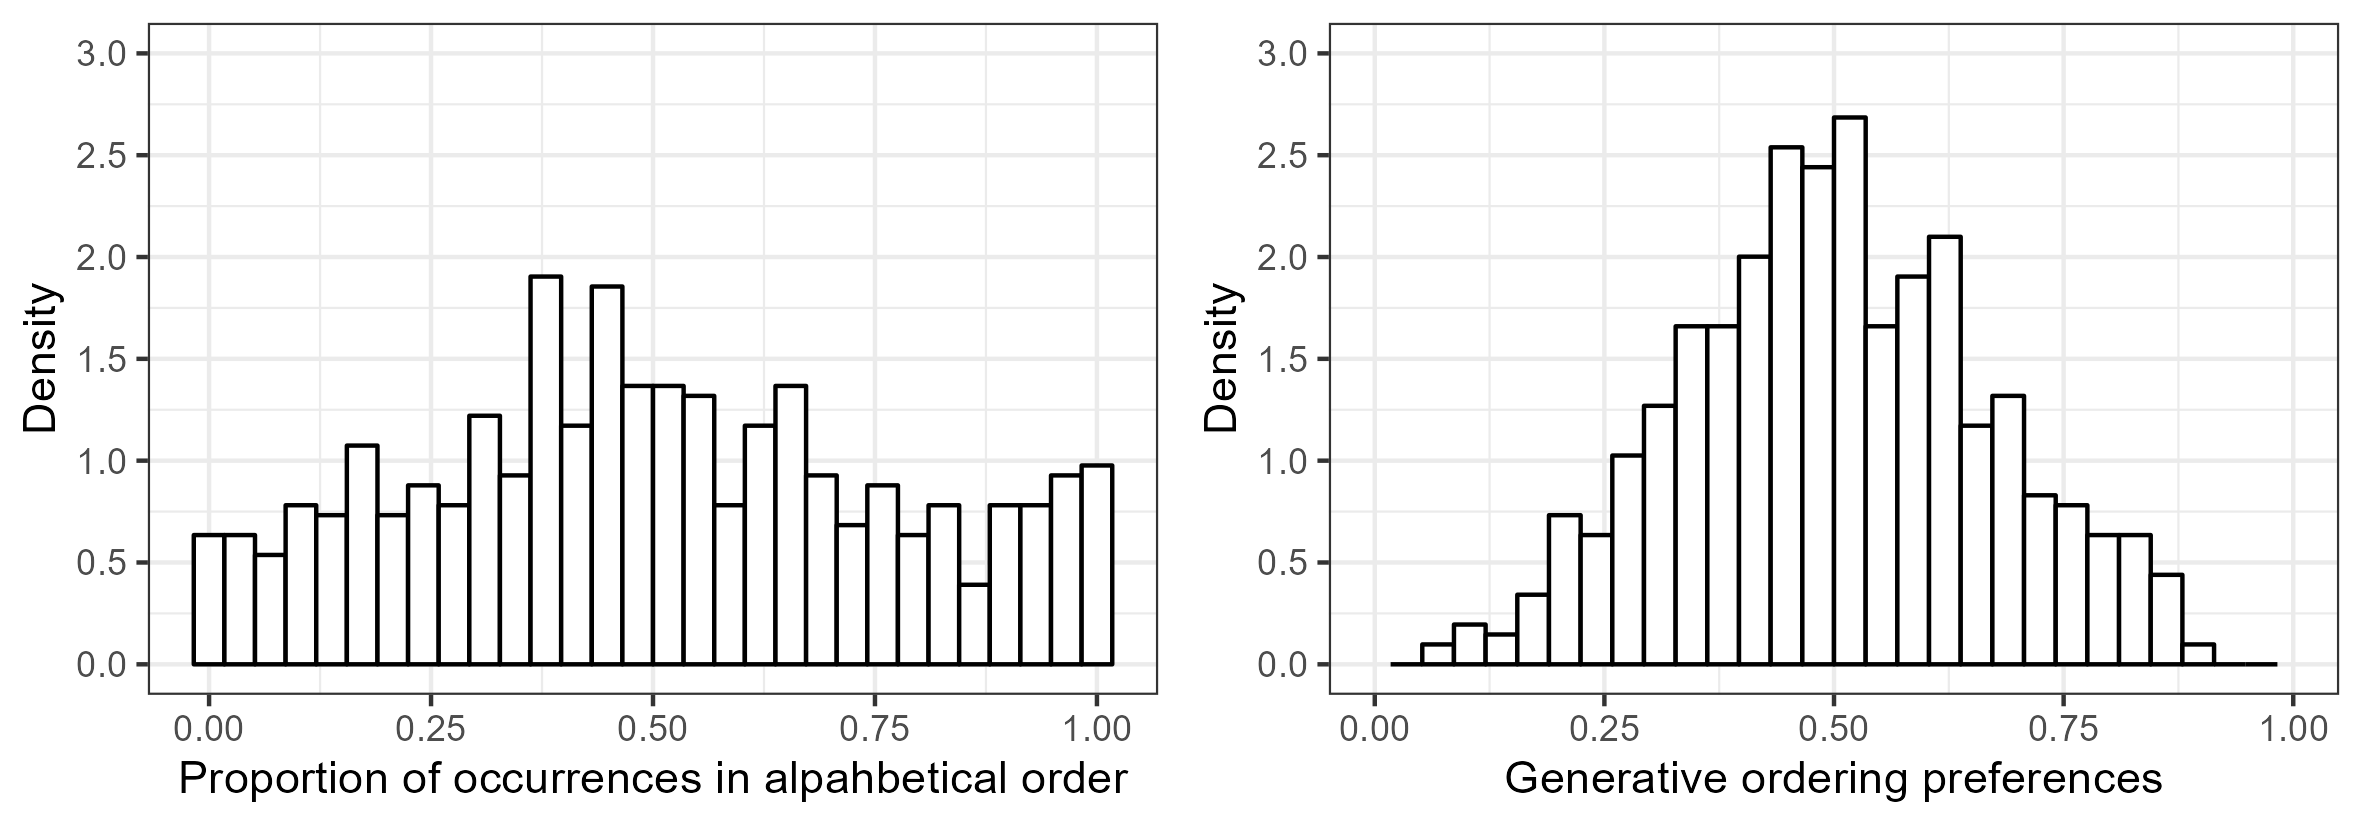
\includegraphics[width=1\linewidth]{Figures/corpus_plots} 

}

\caption[The left plot is a plot of the observed orderings of binomials in the corpus data from @morganModelingIdiosyncraticPreferences2015, the right is the plot of the generative preferences of binomials in the same corpus]{The left plot is a plot of the observed orderings of binomials in the corpus data from @morganModelingIdiosyncraticPreferences2015, the right is the plot of the generative preferences of binomials in the same corpus. The x-axis is proportion of occurrences in alphabetical order and the y-axis is the probability density.}\label{fig:corpusplot1}
\end{figure}
\end{CodeChunk}

\hypertarget{model}{%
\section{Model}\label{model}}

Following Morgan \& Levy (2016b), we use a 2-alternative iterated
learning paradigm. At very step, learners hear N tokens with some in
alphabetical (AandB) and some in nonalphabetical (BandA) order. After
hearing a single token, learners compute \(P(S_i = AandB|S_p)\) and
update their beliefs about prior probability of the ordering for a given
binomial, \(P(S_i)\). The size of the update is proportional to how
probable the learner believes the binomial ordering is.

After hearing a token, learners compute \(P(S_i = AandB|S_p)\)
proportional to \(P(S_i) \cdot P(S_i \to S_p)\). \(P(S_i \to S_p)\) is a
fixed noise parameter, which we will call \(P(noise)\). \(P(noise)\)
represents the probability of the perceived binomial ordering being
swapped by the learner (i.e., AandB being swapped to BandA or vice
versa). \(P(S_i)\) represents the learner's belief of the probability of
the intended order of the binomial.

To initialize \(P(S_i)\) before the learner hears any data, we used the
mean and concentration parametrization of the beta distribution. The
mean (\(\mu\)) represents the expectation of the distribution (the mean
value of draws from the distribution). The concentration parameter
(\(\nu\)) describes how dense the distribution is.

Before the learner hears any data, \(\mu\) is equal to the generative
preference for the binomial (taken from Morgan \& Levy, 2016b). \(\nu\)
is a free parameter, set to 10 for all simulations in this
paper.\footnote{Changing \(\nu\) does not qualitatively change the
  pattern of the results for any simulations in the paper, as long as
  it's greater than 2.}

We then use \(P(S_i)\) and \(P(noise)\) to compute \(P(S_i|S_p)\). If
the perceived binomial is alphabetical (AandB), we compute the
unnormalized probability of the alphabetical and nonalphabetical
orderings according to the below equations.

\begin{equation}
\label{eq:praw}
P_{raw}(S_i = AandB|S_p = AandB) = P(S_i = AandB) \cdot (1 -  P(noise))
\end{equation}

\begin{equation}
\label{eqprawtwo}
P_{raw}(S_i = BandA|AandB) = 1 - P(S_i = AandB) \cdot P(noise)
\end{equation}

In particular, \(P(S_i = AandB)\) = \(\mu\), where \(\mu\) =
\(\alpha_1\) / (\(\alpha_1 + \alpha_2\)) in the pseduco count
parametrization. In fact, for updating we use the pseudocount
parametrization, where \(\alpha_1 = \mu \cdot \nu\) and
\(\alpha_2 = 1-\mu \cdot \nu\).

After calculating the unnormalized (raw) probabilities, they are then
normalized:

\begin{equation}
\label{eq:phatalpha}
\hat{P}(\alpha) = \frac{P_{raw}(S_i = AandB|S_p = AandB)}{P_{raw}(S_i = AandB | S_p = AandB) + P_{raw}(S_i = BandA|S_p = AandB)}
\end{equation}

\begin{equation}
\label{eq:phatnotalpha}
\hat{P}(\neg\alpha) = 1 - \hat{P}(\alpha)
\end{equation}

We then update \(\alpha_1'\) and \(\alpha_2'\) to be used as the
pseudocount parameters of \(P(S_i)\) when the learner hears the next
token. This update is done according to the following equation (note
that for the update we use the pseudo count parametrization):

\begin{equation}
\label{eq:alpha1}
\alpha_1' = \alpha_1 + \hat{P}(\alpha)
\end{equation}

\begin{equation}
\label{eq:alpha2}
\alpha_2' = \alpha_2 + \hat{p}(\neg\alpha)
\end{equation}

When the learner hears the next token, they use \(\alpha_1'\) and
\(\alpha_2'\) to compute \(P(S_i)\). Note that when learner hear AandB,
they update their beliefs about the probability of both the
alpahabetical \emph{and} nonalphabetical forms of the binomial.

When the learner is done hearing N tokens and updating their beliefs of
\(P(S_i)\) for a given binomial, they then produce N tokens for the next
generation of learners. These are generated binomially, where
\(\theta_1 = P(S_i=AandB)\) is the inferred probability of the
alphabetical form of a given binomial:

\begin{equation}
\label{eq:binomialProd}
P(x_1|\theta_1) = \binom{N}{x_1} \theta^{x_1} (1-\theta_1)^{N-x_1}
\end{equation}

When producing each token, there is also a possibility that the speaker
makes an error and produces an unintended ordering of the binomial. In
order to model this, the speaker produces a token in the unintended
order with probability \(P(SpeakerNoise)\). This is a fixed parameter in
the model and remains constant across binomials and
generations.\footnote{All code and results can be found publicly
  available here:
  \url{https://github.com/znhoughton/Noisy-Channel-Iterated-Learning}}

This process continues iteratively for \(ngen\) generations.

\hypertarget{results}{%
\section{Results}\label{results}}

\hypertarget{speaker-vs-listener-noise}{%
\subsection{Speaker vs Listener Noise}\label{speaker-vs-listener-noise}}

First we demonstrate that frequency-dependent regularization does not
arise when there is no listener or speaker noise.\footnote{All code and
  results can be found publicly available here:
  \url{https://github.com/znhoughton/Noisy-Channel-Iterated-Learning}}
Instead we see convergence to the prior, which is expected. That is,
Griffiths \& Kalish (2007) demonstrated that when learners sample from
the posterior, as the number of iterations increases, the stationary
distribution converges to the prior. In other words, without any noise,
each generation of learners produces data that is more and more similar
to the prior, until convergence is reached (Figure
\ref{fig:noNoisePlot}).

\begin{CodeChunk}
\begin{figure}[tb]

{\centering 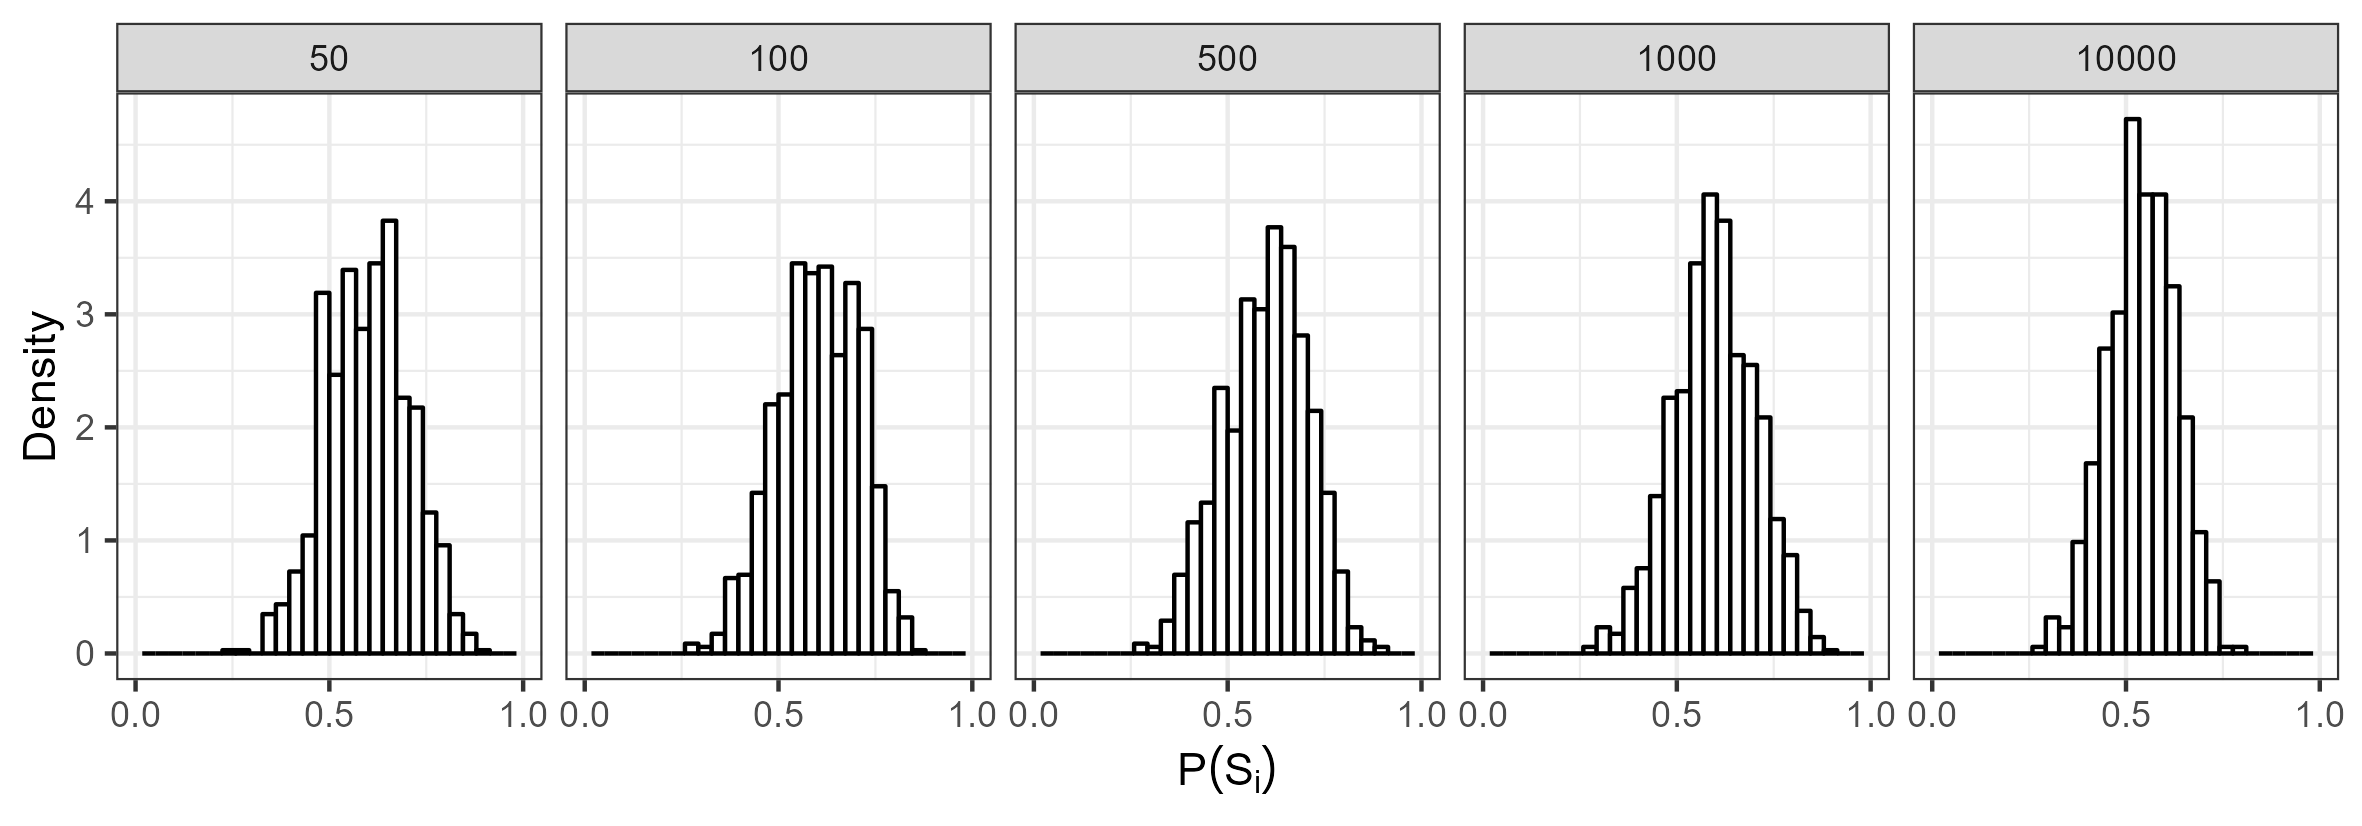
\includegraphics[width=1\linewidth]{Figures/noNoise} 

}

\caption[A plot of the distribution of simulated binomials at the 500th generation, varying in frequency]{A plot of the distribution of simulated binomials at the 500th generation, varying in frequency. The top value represents N. On the x-axis is the predicted probability of producing the binomial in alphabetical form. On the y-axis is probability density. Speaker and listener noise was set to 0. The generative preference was 0.6, and nu was set to 10. 1000 chains were run. Note that there is no frequency-dependent regularization apparent.}\label{fig:noNoisePlot}
\end{figure}
\end{CodeChunk}

However, when we introduce noise (Figure \ref{fig:regularizationplot1}),
we see that the model can predict frequency-dependent regularization
across generations.

\begin{CodeChunk}
\begin{figure}[tb]

{\centering 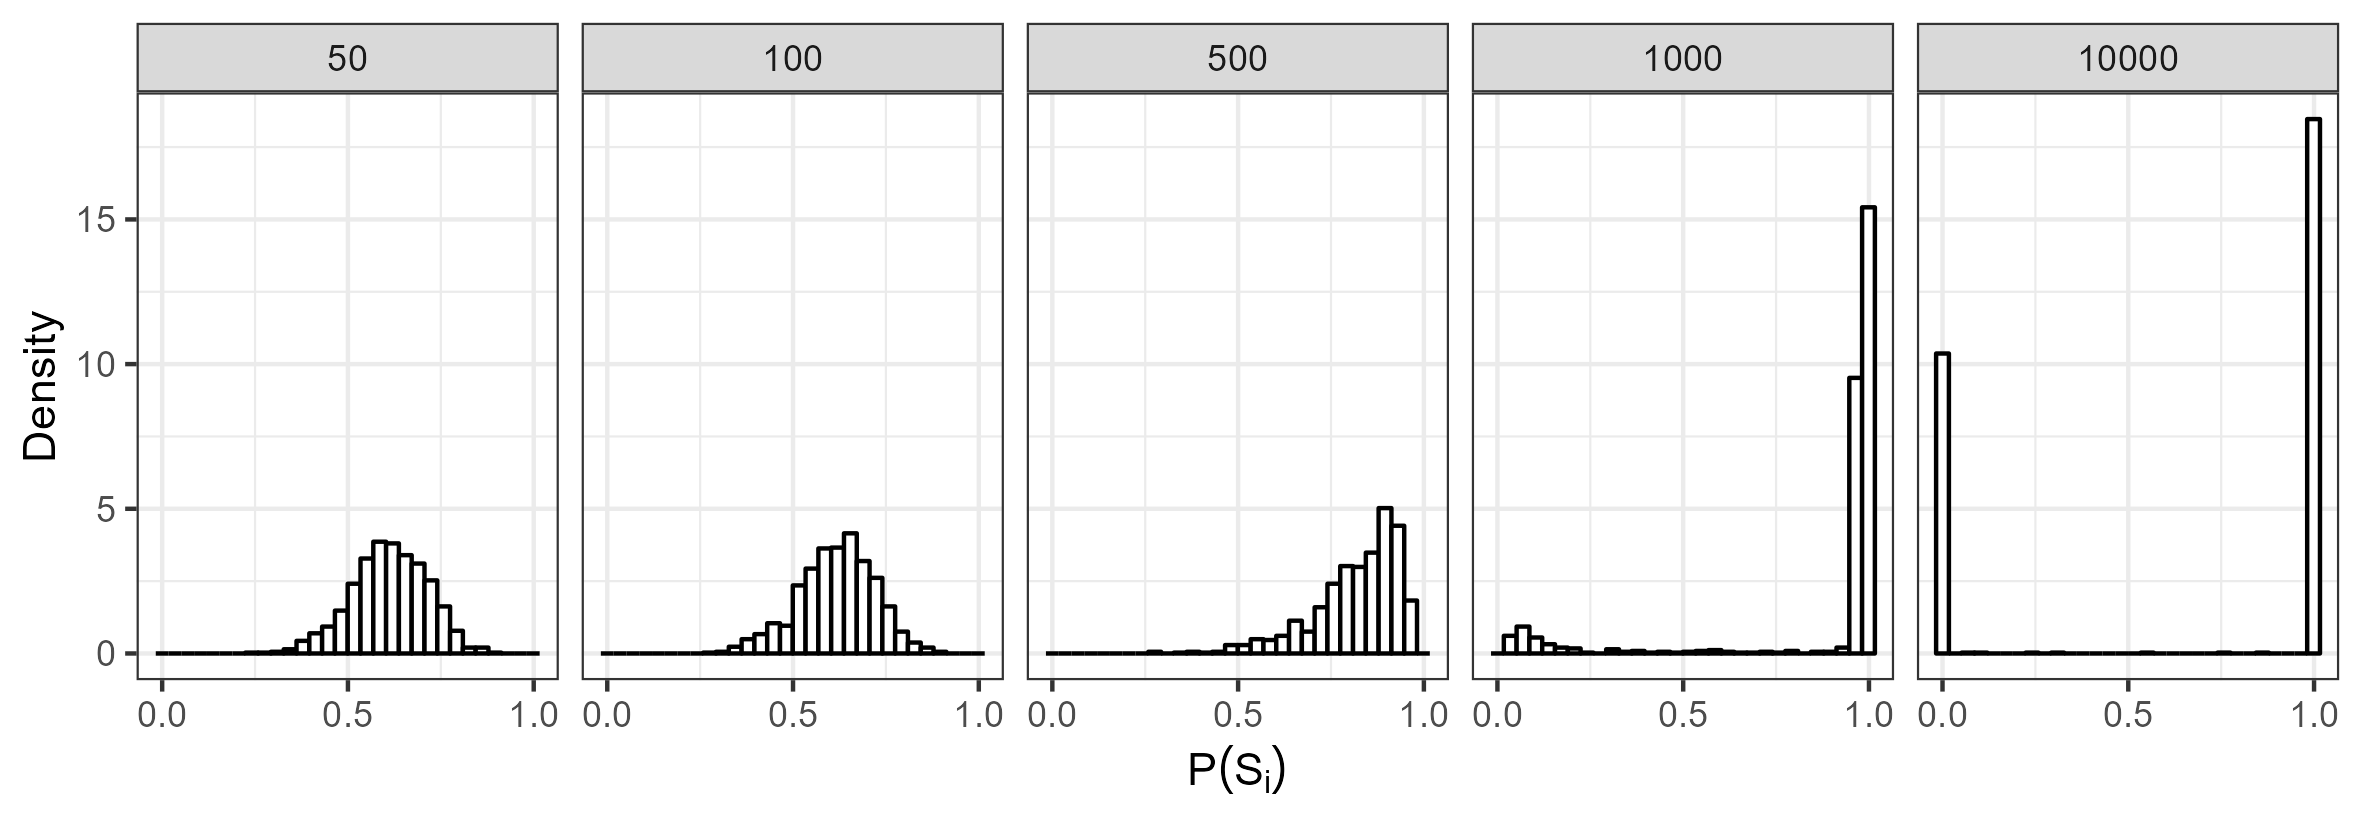
\includegraphics[width=1\linewidth]{Figures/speaker_noise_001_listener_01} 

}

\caption[A plot of the distribution of simulated binomials at the 500th generation, varying in frequency]{A plot of the distribution of simulated binomials at the 500th generation, varying in frequency. The top value represents N. On the x-axis is the predicted probability of producing the binomial in alphabetical form. On the y-axis is probability density. Speaker noise was set to 0.001, listener noise was set to 0.01, the generative preference was 0.6, and nu was set to 10. 1000 chains were run. Note how for the binomials with large N, the ordering preferences tend to be more extreme.}\label{fig:regularizationplot1}
\end{figure}
\end{CodeChunk}

Further, the disparity of the noise affects the rate of regularization.
Increased noise results in weaker regularization (i.e., less
regularization for lower frequency items, see Figure
\ref{fig:absolutediff}), however a larger relative difference between
the speaker and listener noise parameters increases both the strength
and the speed of the regularization (see Figure
\ref{fig:fasterslowerreg}).

\begin{CodeChunk}
\begin{figure}[tb]

{\centering 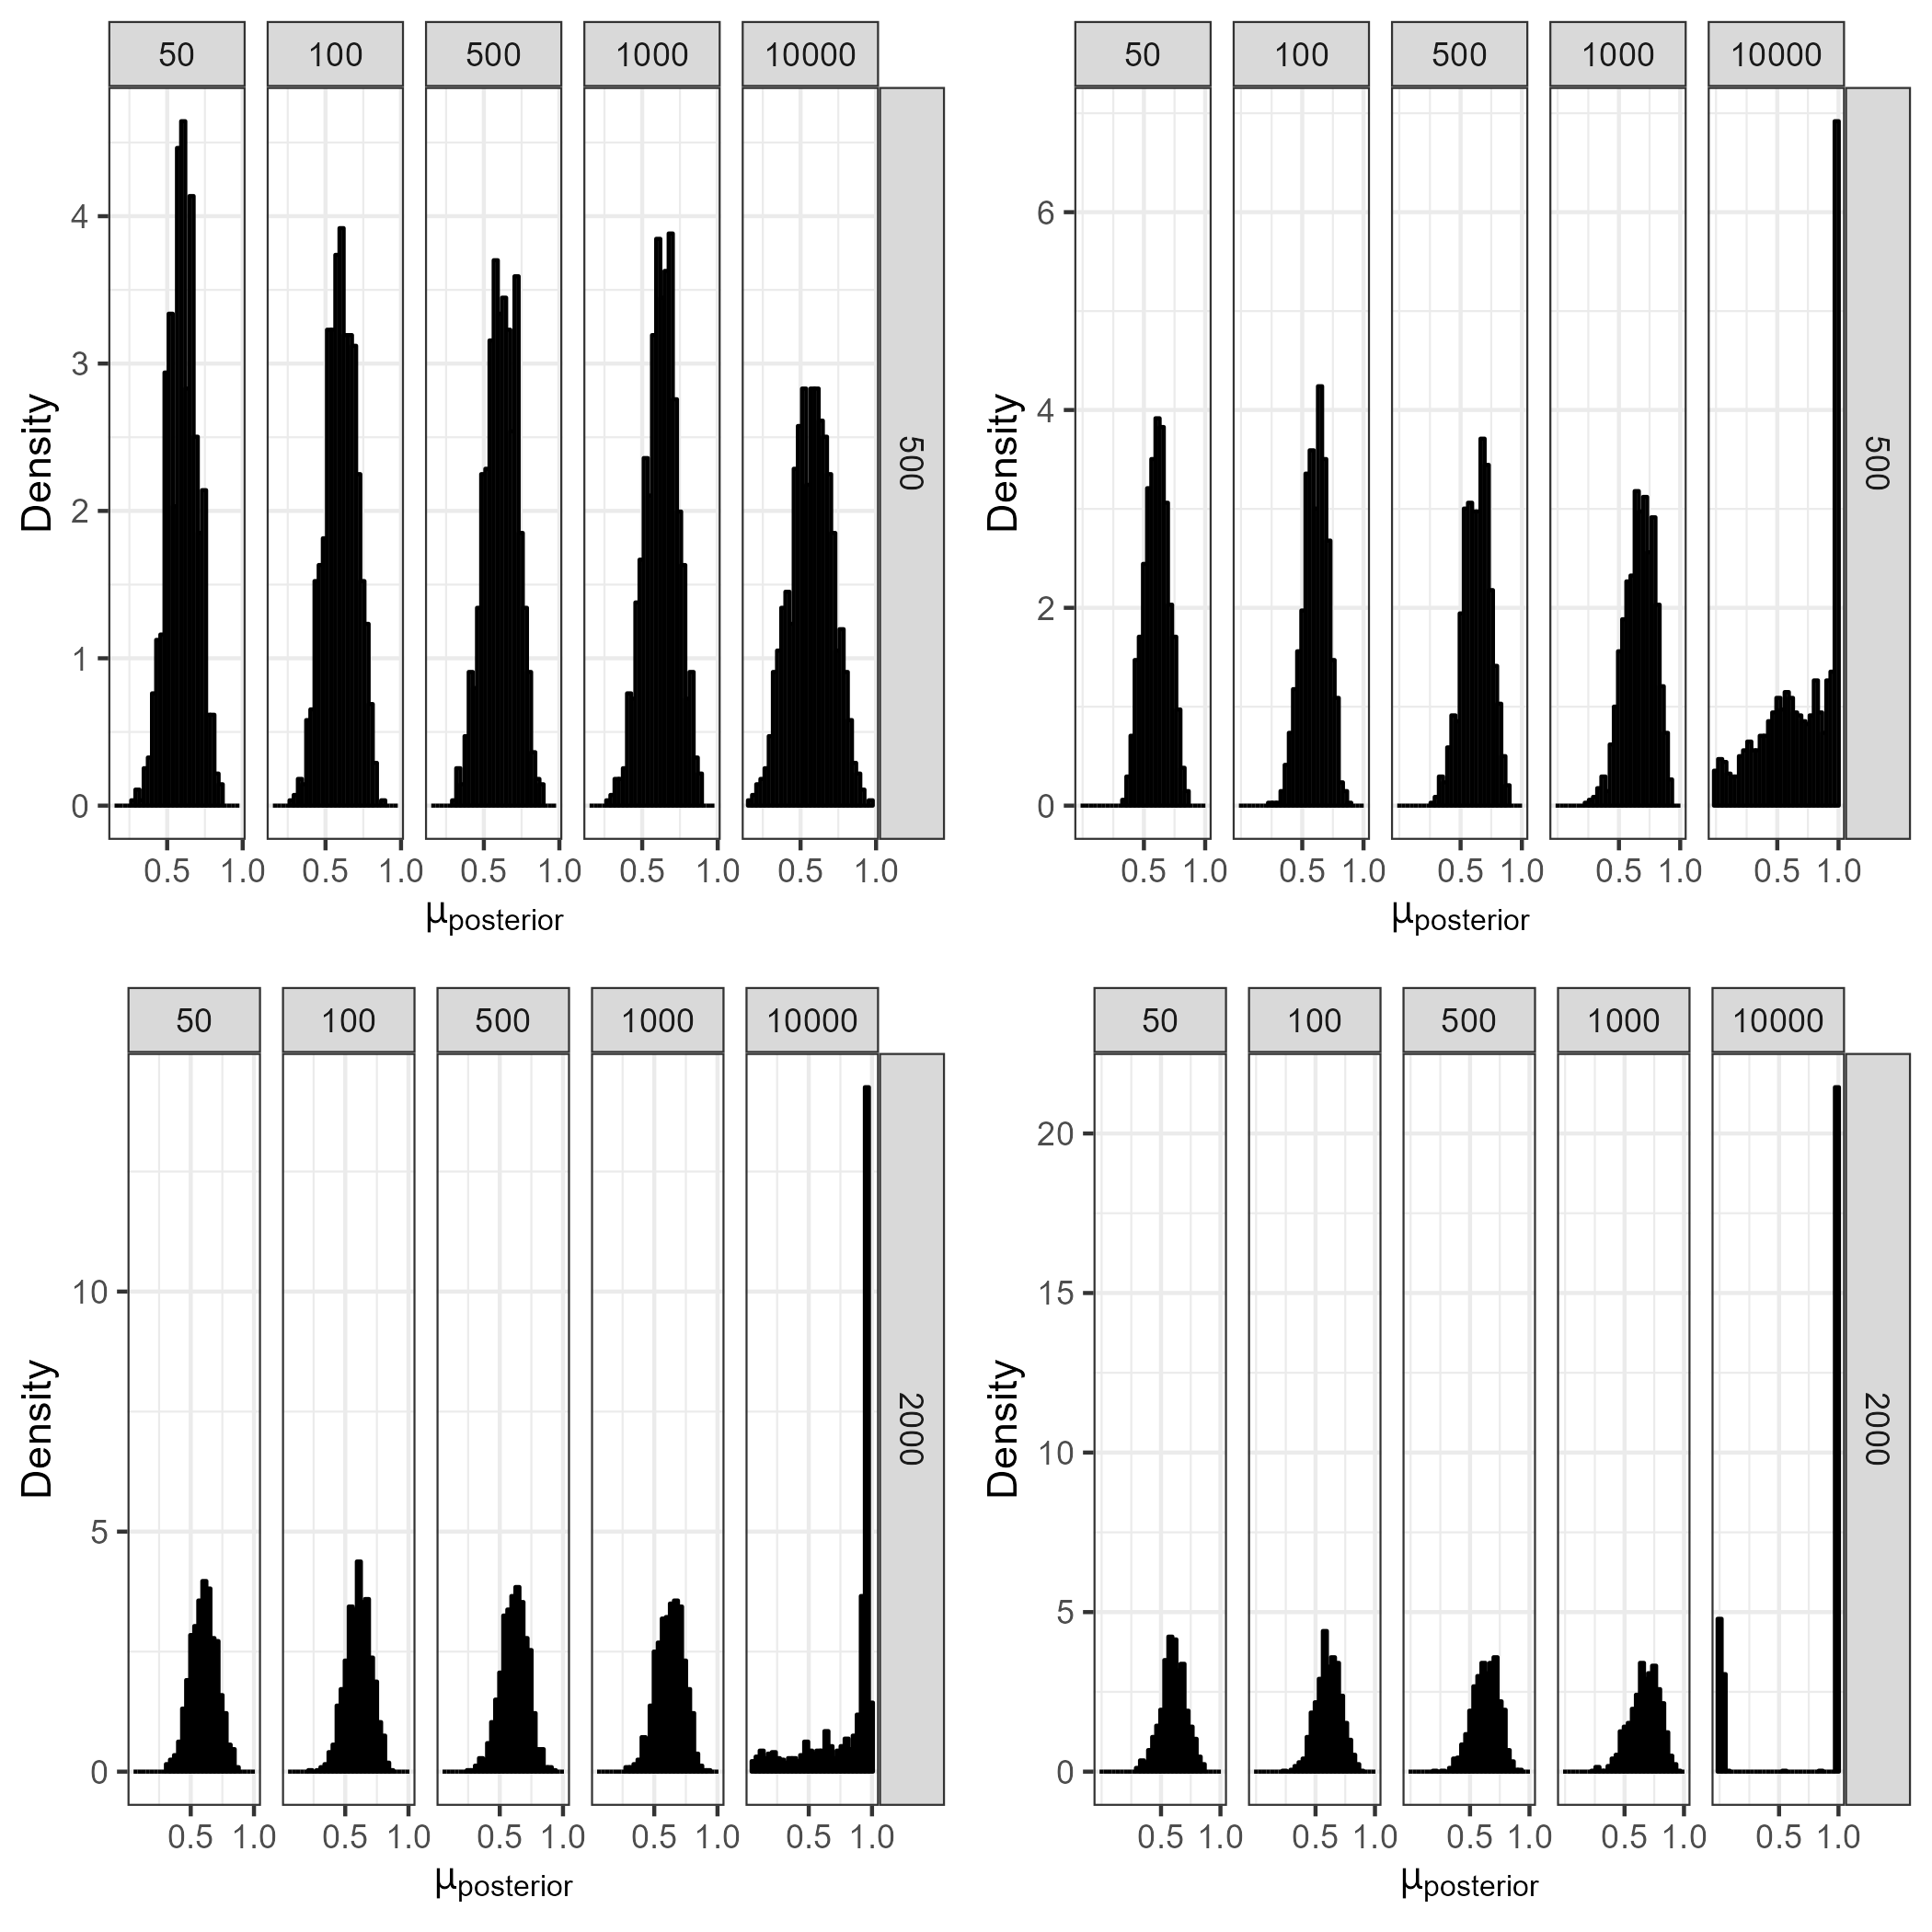
\includegraphics[width=1\linewidth]{Figures/fasterSlowerReg} 

}

\caption[A plot of simulations with different noise parameters at 500 (top plots) and 2000 (bottom plots) generations]{A plot of simulations with different noise parameters at 500 (top plots) and 2000 (bottom plots) generations. For the left plots, the speaker noise was set to 0.009 and the listener noise parameter was set to 0.01. For the right plots, the speaker noise was set to 0.0075 and the listener noise parameter was set to 0.01. For both plots, the generative preference was set to 0.6 and nu was set to 10.}\label{fig:fasterslowerreg}
\end{figure}
\end{CodeChunk}

\begin{CodeChunk}
\begin{figure}[tb]

{\centering 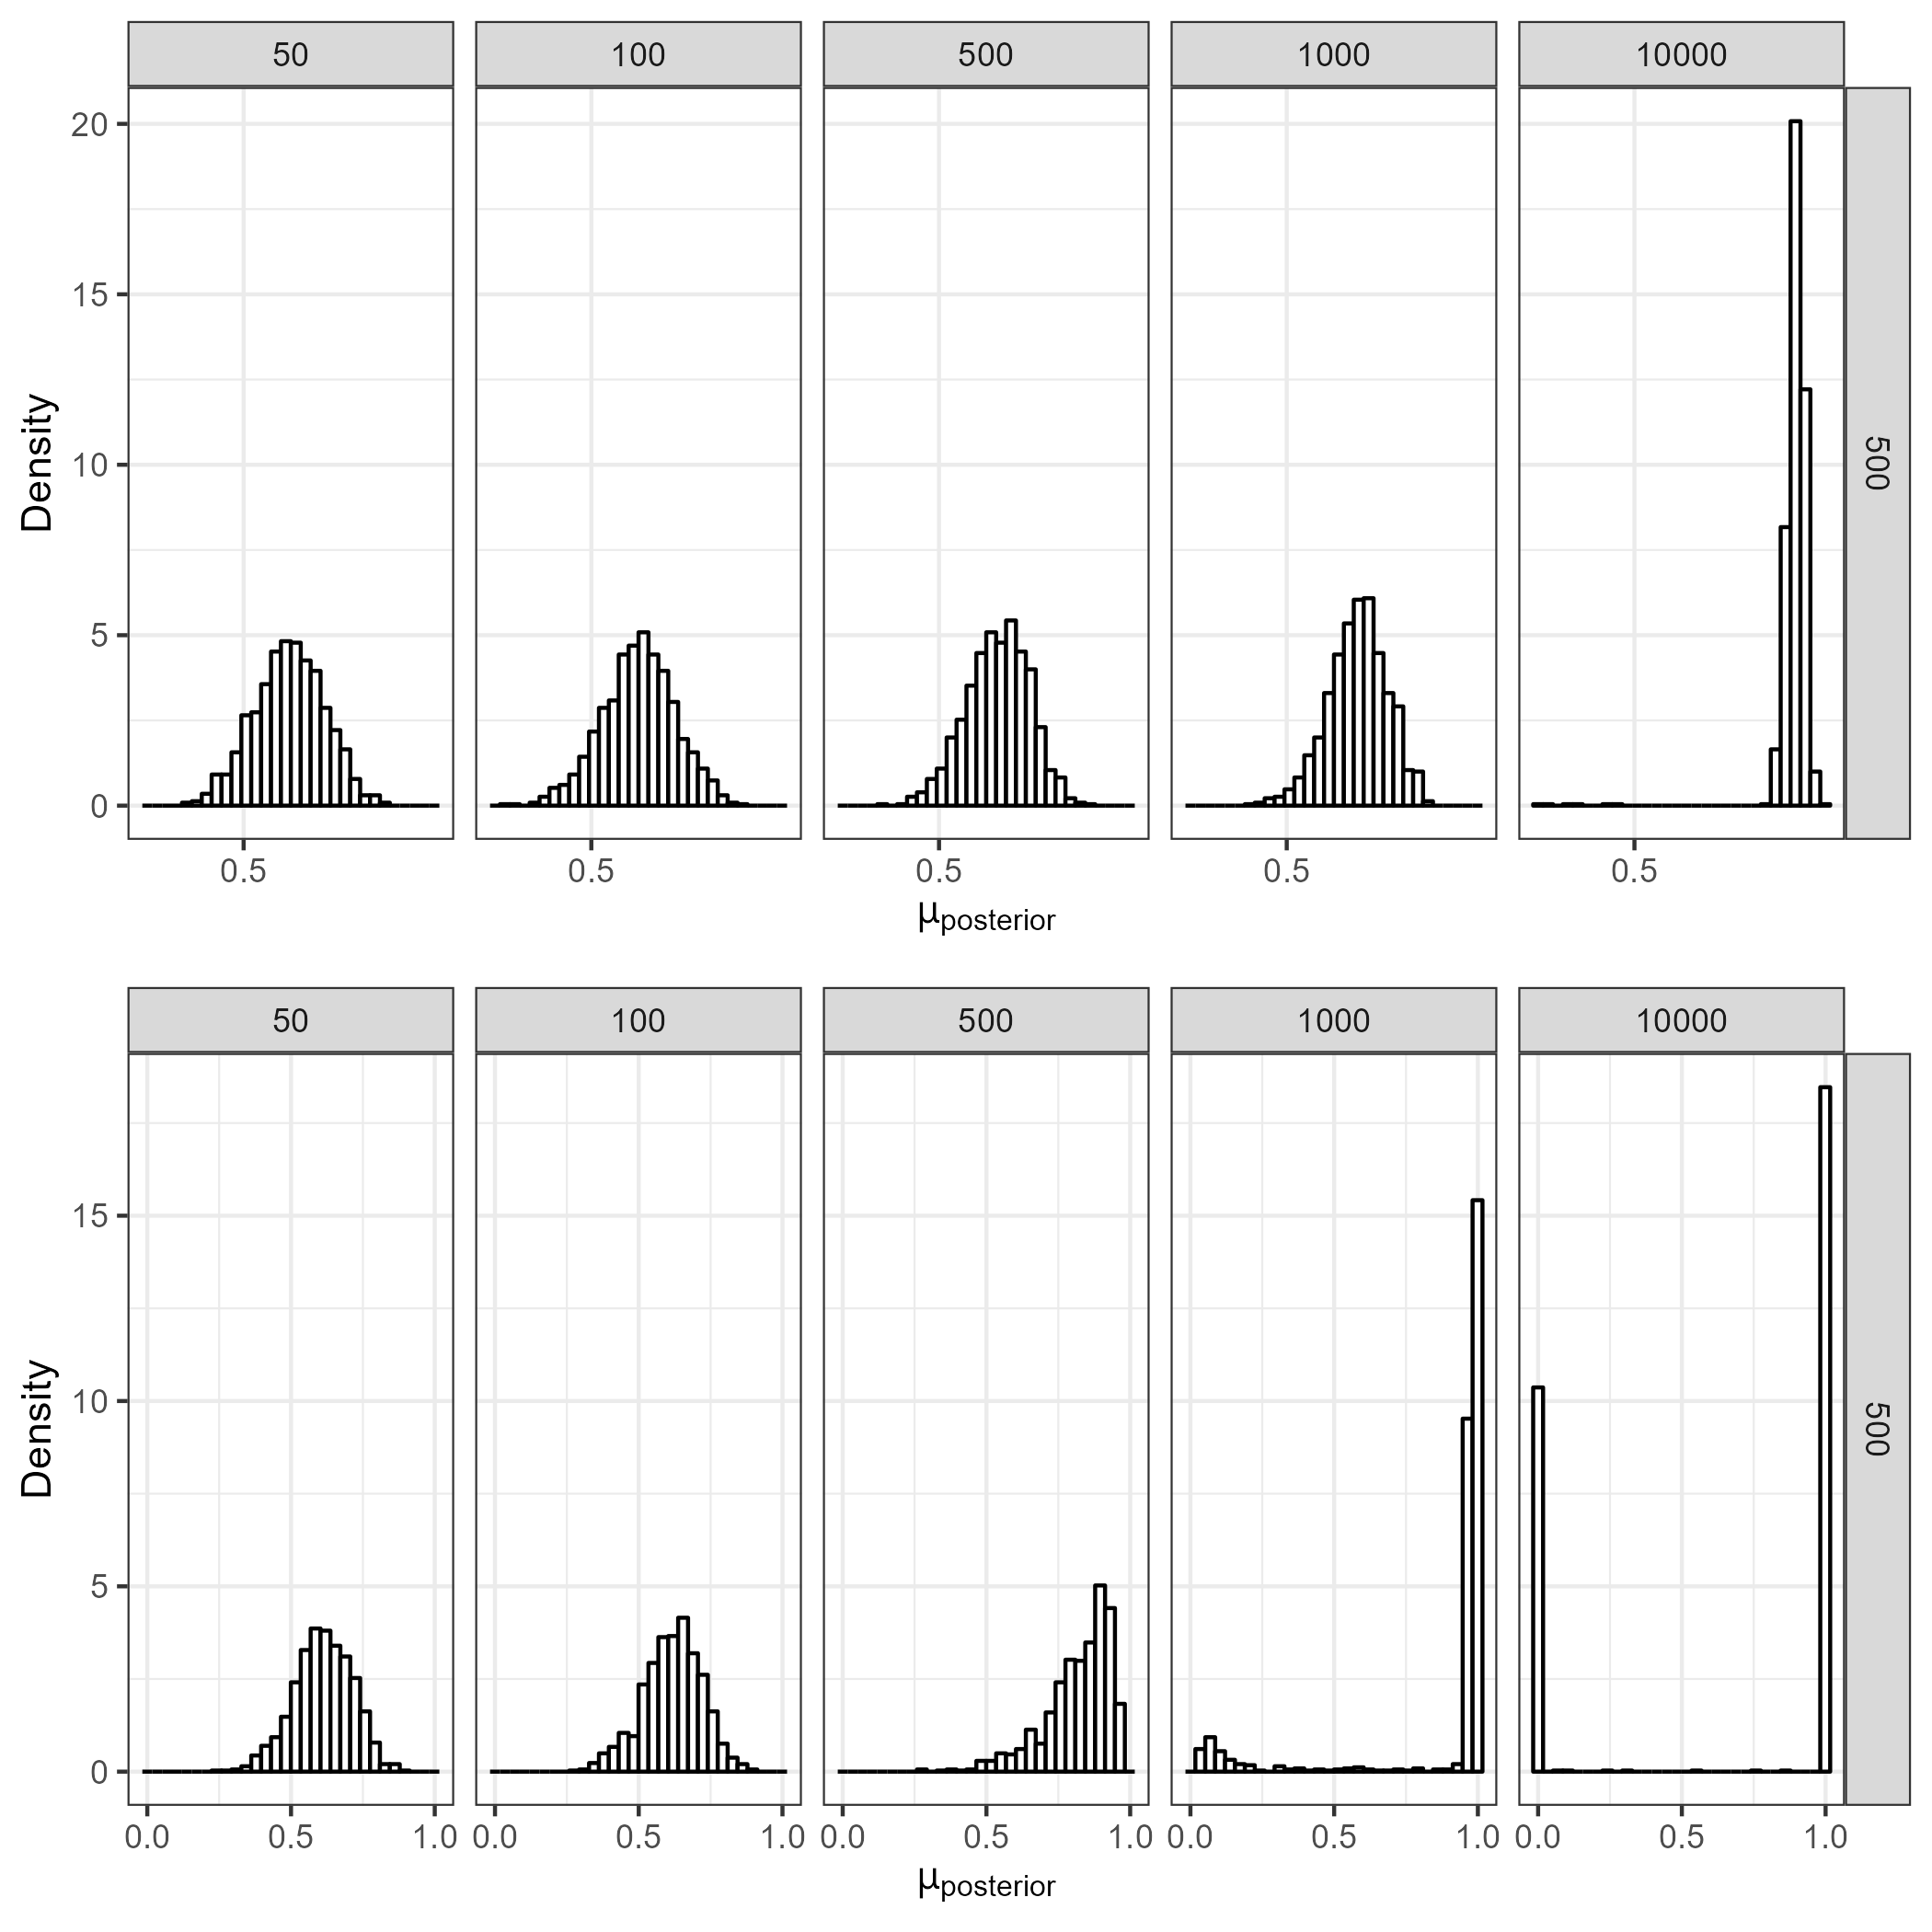
\includegraphics[width=1\linewidth]{Figures/absolute_matters} 

}

\caption[A plot of simulations with different noise parameters, but the same relative difference between the speaker and listener noise parameters]{A plot of simulations with different noise parameters, but the same relative difference between the speaker and listener noise parameters. The top plot For the top plot, the speaker noise was set to 0.091 and listener noise was set to 0.1. For the bottom plot, the speaker noise was set to 0.001 and listener noise was set to 0.01. Note that the relative difference between the listener and speaker noise parameters for both plots was the same (0.009).}\label{fig:absolutediff}
\end{figure}
\end{CodeChunk}

Interestingly this regularization disappears if the listener's noise
parameter is less than or equal to the speaker's noise parameter (Figure
\ref{fig:regularizationplot2}).

\begin{CodeChunk}
\begin{figure}[tb]

{\centering 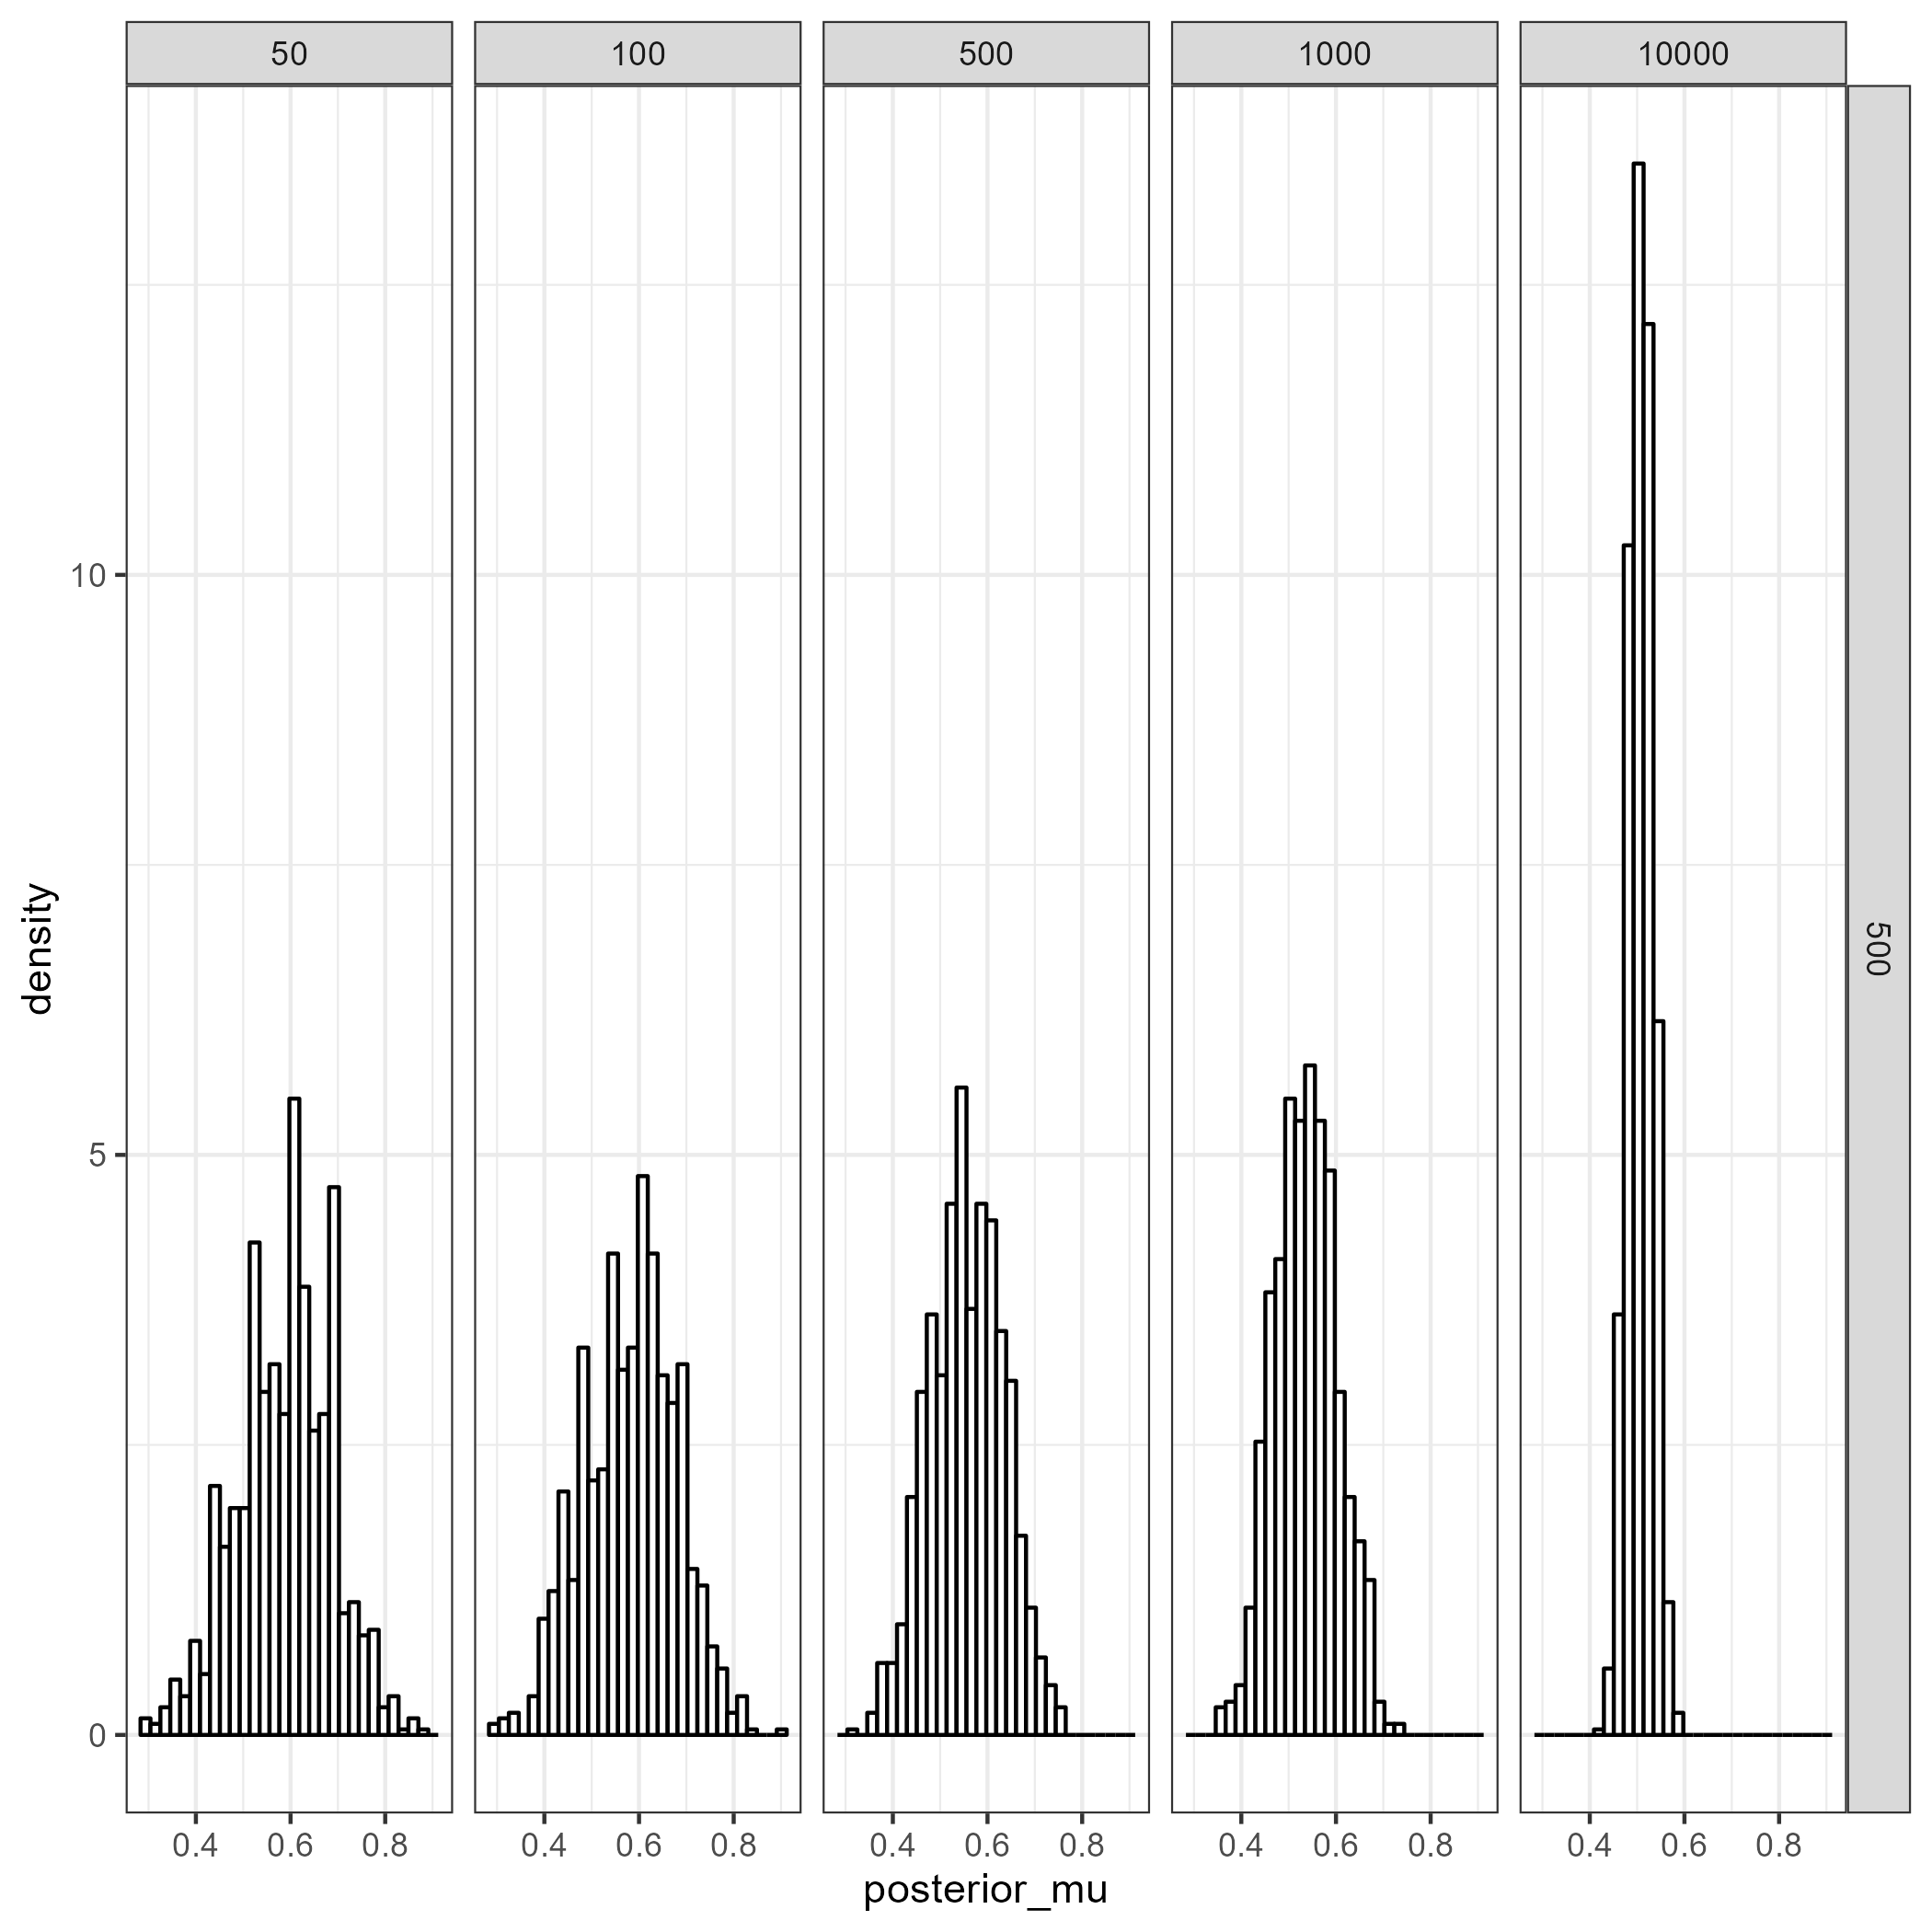
\includegraphics[width=1\linewidth]{Figures/speaker_noise_01_listener_001} 

}

\caption[A plot of the distribution of simulated binomials at the 500th generation, varying in frequency]{A plot of the distribution of simulated binomials at the 500th generation, varying in frequency. The top value represents N. On the x-axis is the predicted probability of producing the binomial in alphabetical form. On the y-axis is probability density. Speaker noise was set to 0.01, listener noise was set to 0.001, the generative preference was 0.6, and nu was set to 10. 1000 chains were run. Note how regularization does not appear to be present in this graph.}\label{fig:regularizationplot2}
\end{figure}
\end{CodeChunk}

It is useful to revisit here what the speaker and listener noise
parameters represent. The speaker noise parameter is how often the
speaker produces an error and the listener noise parameter is the
listeners' belief of how noisy the environment is. Framed this way, it
is perhaps unsurprising that we do not see regularization when the
parameters equal eachother, since they essentially cancel eachother out
(everytime a speaker makes an error, the listener is accounting for it,
thus we get convergence to the prior).

Thus our model makes a novel prediction: In order to account for
frequency-dependent regularization, listeners must be inferring more
noise than speakers are actually producing (according to our model).

\hypertarget{corpus-data}{%
\subsection{Corpus Data}\label{corpus-data}}

Finally, we now demonstrate that our model also predicts the
language-wide distribution of binomial preference strengths seen in the
corpus data. Specifically, we show that with \(\nu\) set to 10, listener
noise set to 0.02, and speaker noise set to 0.005, our model does a
pretty good job of approximating the distribution in the corpus data
(See Figure \ref{fig:corpusourmodel}).

\begin{CodeChunk}
\begin{figure}[tb]

{\centering 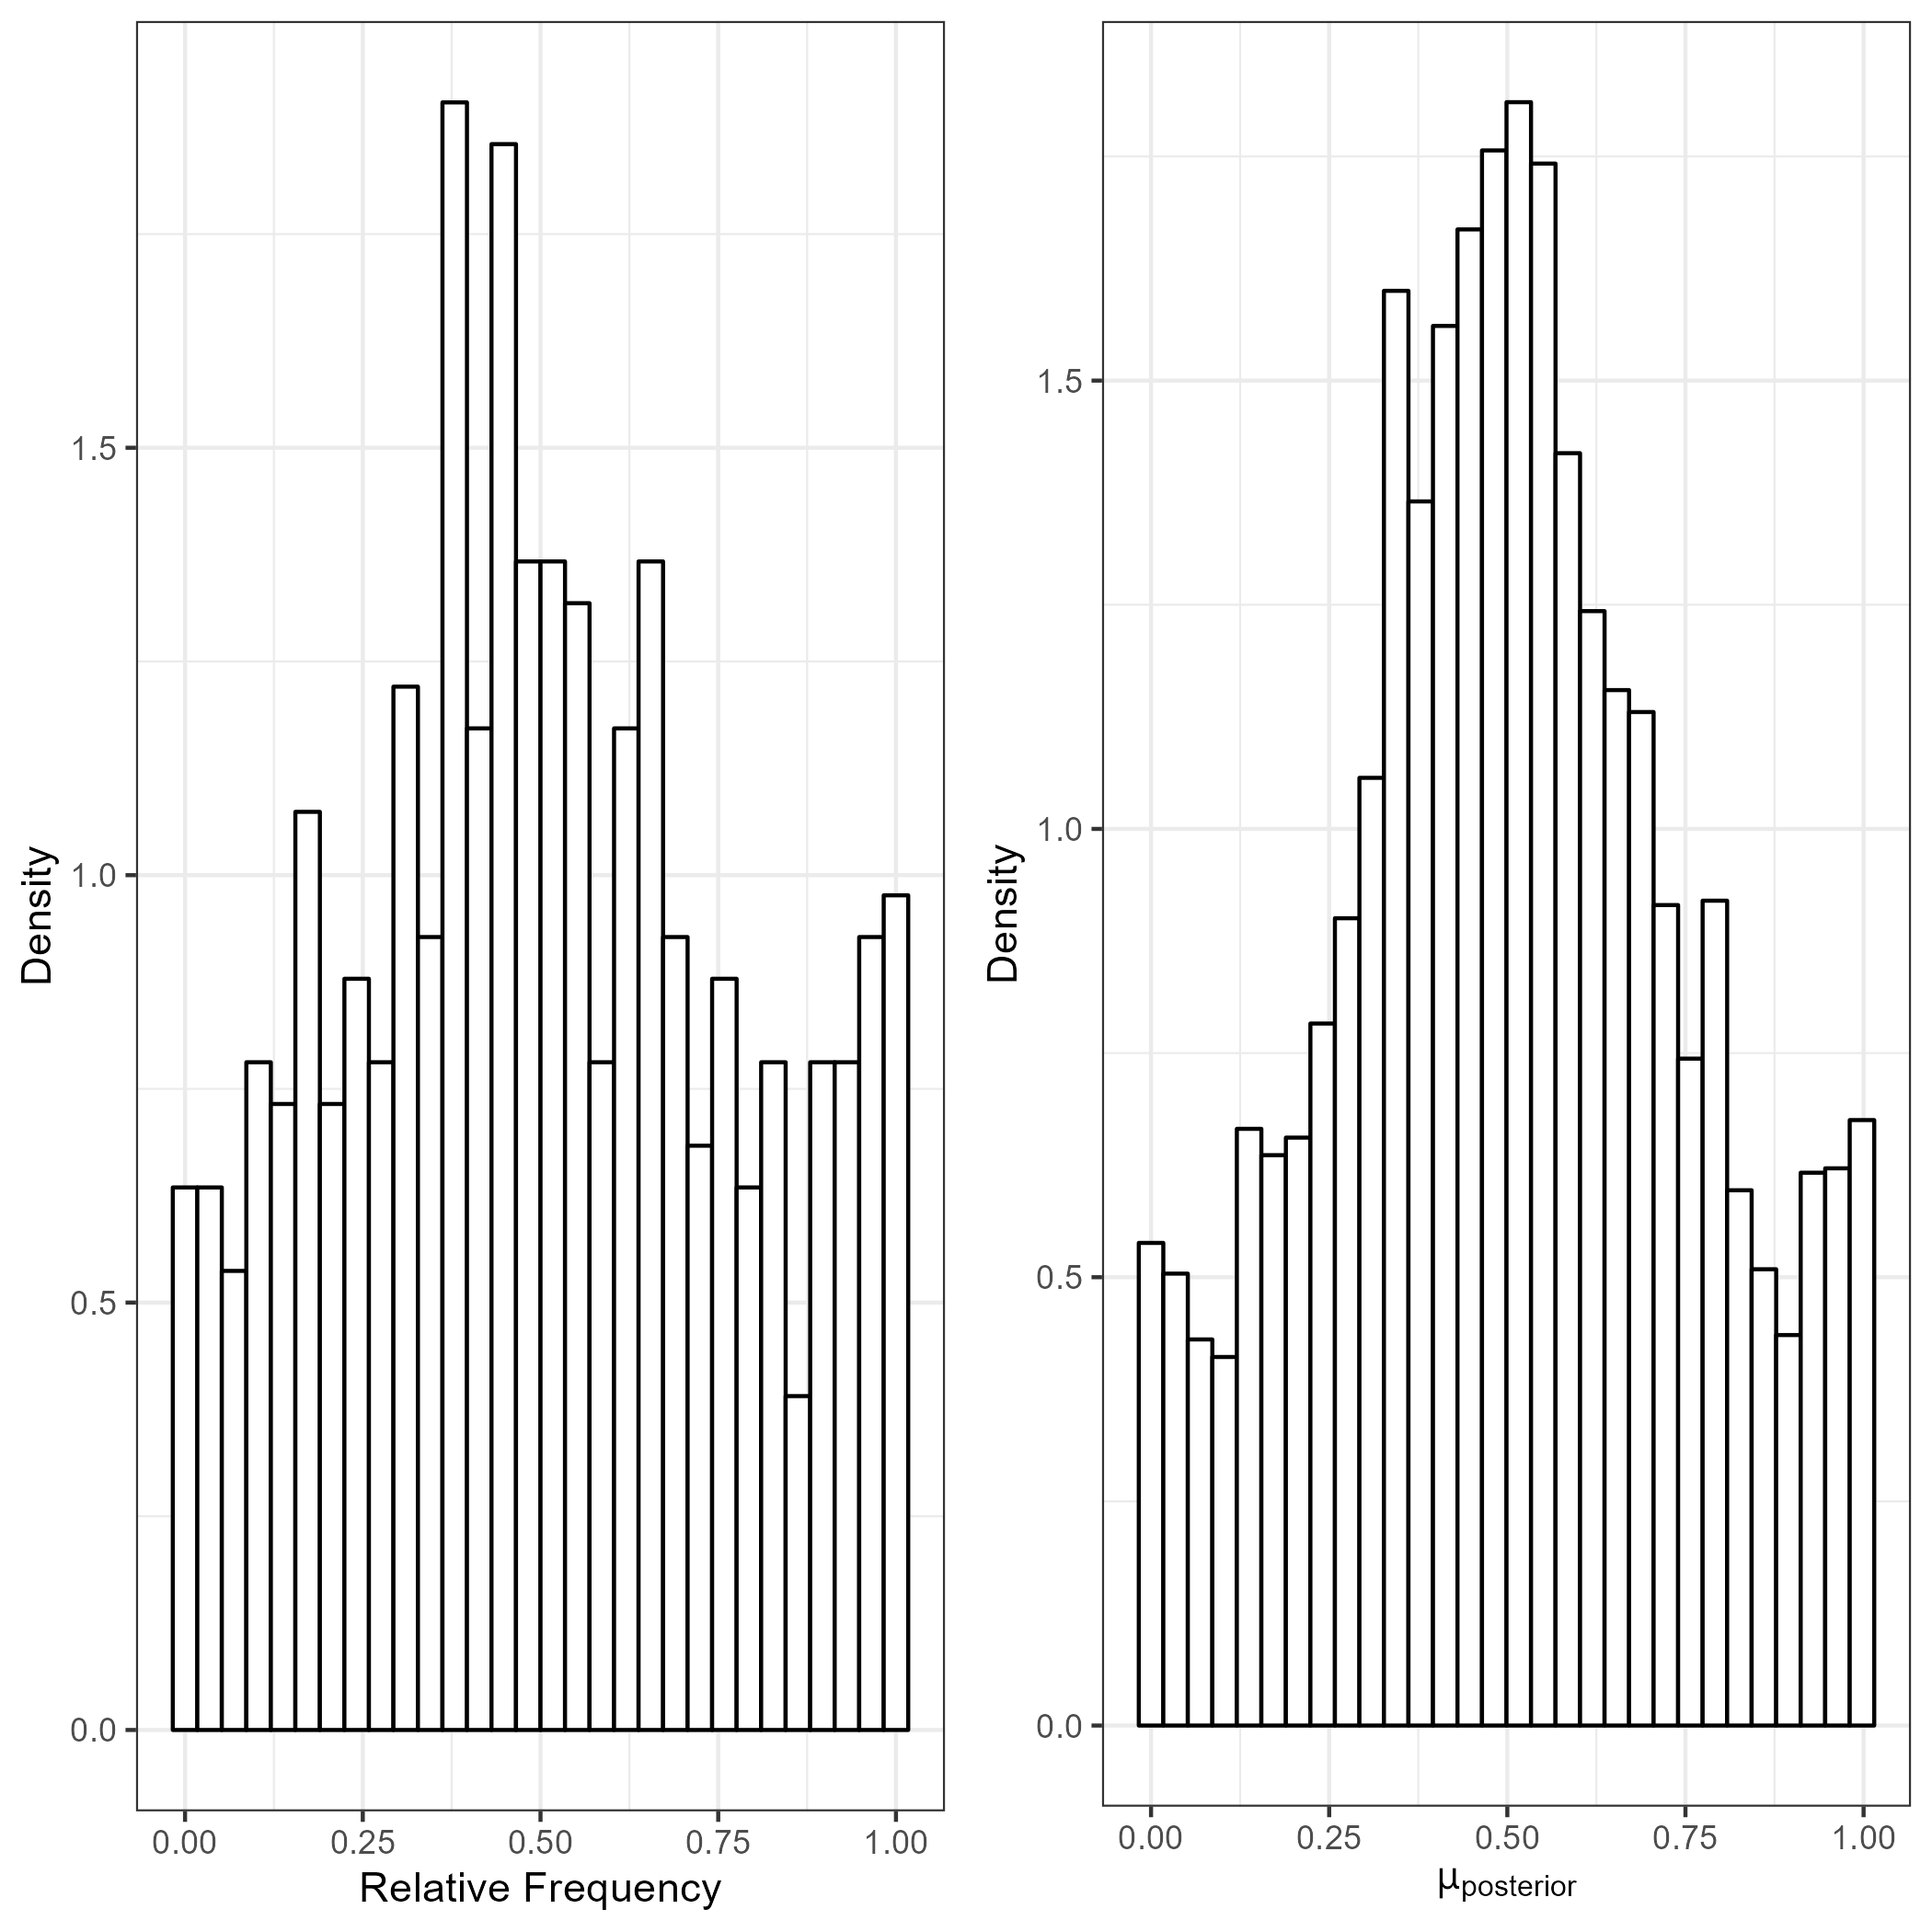
\includegraphics[width=1\linewidth]{Figures/corpus_plot_and_ours} 

}

\caption[A plot of the distribution of ordering preferences after 500 generations of our iterated learning model (left) and the distribution of ordering preferences in the corpus data from Morgan \& Levy (2015)]{A plot of the distribution of ordering preferences after 500 generations of our iterated learning model (left) and the distribution of ordering preferences in the corpus data from Morgan \& Levy (2015). For our simulations, the binomial frequencies and generative preferences were matched with the corpus data. $
u$ was set to 10, listener noise was set to 0.02, and speaker noise was set to 0.005.}\label{fig:corpusourmodel}
\end{figure}
\end{CodeChunk}

\hypertarget{conclusion}{%
\section{Conclusion}\label{conclusion}}

Our results demonstrate the frequency-dependent regularization emerges
from a noisy-channel processing model (Gibson et al., 2013) in an
iterative-learning paradigm (Morgan \& Levy, 2016b; Reali \& Griffiths,
2009) when listeners assume more noise in the environment than the
speakers actually produce.

Further our results suggest that in order to account for
frequency-dependent regularization, listeners are inferring more noise
than speakers are producing. An interesting avenue for future research
is whether this prediction is born out in experimental work.

\hypertarget{references}{%
\section{References}\label{references}}

\setlength{\parindent}{-0.1in} 
\setlength{\leftskip}{0.125in}

\noindent

\hypertarget{refs}{}
\begin{CSLReferences}{1}{0}
\leavevmode\vadjust pre{\hypertarget{ref-feltyMisperceptionsSpokenWords}{}}%
Albert Felty, R., Buchwald, A., Gruenenfelder, T. M., \& Pisoni, D. B.
(2013). Misperceptions of spoken words: Data from a random sample of
american english words. \emph{The Journal of the Acoustical Society of
America}, \emph{134}(1), 572--585.

\leavevmode\vadjust pre{\hypertarget{ref-benor2006}{}}%
Benor, S. B., \& Levy, R. (2006). The chicken or the egg? A
probabilistic analysis of english binomials. \emph{Language}, 233278.

\leavevmode\vadjust pre{\hypertarget{ref-ganongPhoneticCategorizationAuditory1980}{}}%
Ganong, W. F. (1980). Phonetic categorization in auditory word
perception. \emph{Journal of Experimental Psychology: Human Perception
and Performance}, \emph{6}(1), 110. Retrieved from
\url{https://psycnet.apa.org/record/1981-07020-001}

\leavevmode\vadjust pre{\hypertarget{ref-gibsonNoisy2013}{}}%
Gibson, E., Bergen, L., \& Piantadosi, S. T. (2013). Rational
integration of noisy evidence and prior semantic expectations in
sentence interpretation. \emph{Proceedings of the National Academy of
Sciences}, \emph{110}(20), 8051--8056.
http://doi.org/\href{https://doi.org/10.1073/pnas.1216438110}{10.1073/pnas.1216438110}

\leavevmode\vadjust pre{\hypertarget{ref-griffithsLanguageEvolutionIterated2007}{}}%
Griffiths, T. L., \& Kalish, M. L. (2007). Language evolution by
iterated learning with bayesian agents. \emph{Cognitive Science},
\emph{31}(3), 441--480.
http://doi.org/\href{https://doi.org/10.1080/15326900701326576}{10.1080/15326900701326576}

\leavevmode\vadjust pre{\hypertarget{ref-keshevNoisyBetterRare2021}{}}%
Keshev, M., \& Meltzer-Asscher, A. (2021). Noisy is better than rare:
Comprehenders compromise subject-verb agreement to form more probable
linguistic structures. \emph{Cognitive Psychology}, \emph{124}, 101359.
http://doi.org/\href{https://doi.org/10.1016/j.cogpsych.2020.101359}{10.1016/j.cogpsych.2020.101359}

\leavevmode\vadjust pre{\hypertarget{ref-levyNoisychannel2008}{}}%
Levy, R. (2008). A noisy-channel model of human sentence comprehension
under uncertain input. In (p. 234243). Retrieved from
\url{https://aclanthology.org/D08-1025.pdf}

\leavevmode\vadjust pre{\hypertarget{ref-liu2020}{}}%
Liu, Z., \& Morgan, E. (2020). Frequency-dependent regularization in
constituent ordering preferences. In. Retrieved from
\url{https://www.cognitivesciencesociety.org/cogsci20/papers/0751/0751.pdf}

\leavevmode\vadjust pre{\hypertarget{ref-liu2021}{}}%
Liu, Z., \& Morgan, E. (2021). Frequency-dependent regularization in
syntactic constructions. In (p. 387389). Retrieved from
\url{https://aclanthology.org/2021.scil-1.41.pdf}

\leavevmode\vadjust pre{\hypertarget{ref-morganModelingIdiosyncraticPreferences2015}{}}%
Morgan, E., \& Levy, R. (2015). Modeling idiosyncratic preferences : How
generative knowledge and expression frequency jointly determine language
structure, 1649--1654.

\leavevmode\vadjust pre{\hypertarget{ref-morgan2016}{}}%
Morgan, E., \& Levy, R. (2016a). Abstract knowledge versus direct
experience in processing of binomial expressions. \emph{Cognition},
\emph{157}, 384--402.
http://doi.org/\href{https://doi.org/10.1016/j.cognition.2016.09.011}{10.1016/j.cognition.2016.09.011}

\leavevmode\vadjust pre{\hypertarget{ref-morganFrequencydependentRegularizationIterated2016}{}}%
Morgan, E., \& Levy, R. (2016b). Frequency-dependent regularization in
iterated learning. \emph{The Evolution of Language: Proceedings of the
11th International Conference}.

\leavevmode\vadjust pre{\hypertarget{ref-realiEvolutionFrequencyDistributions2009}{}}%
Reali, F., \& Griffiths, T. L. (2009). The evolution of frequency
distributions: Relating regularization to inductive biases through
iterated learning. \emph{Cognition}, \emph{111}(3), 317--328.
http://doi.org/\href{https://doi.org/10.1016/j.cognition.2009.02.012}{10.1016/j.cognition.2009.02.012}

\end{CSLReferences}

\bibliographystyle{apacite}


\end{document}
